\documentclass[12pt,a4paper,onecolumn]{article}

%%%%%%%%%%%%%%%%%%%%%%%%%%%%%%%%%%%
%          				PACKAGES  				              %
%%%%%%%%%%%%%%%%%%%%%%%%%%%%%%%%%%%

\usepackage[margin=1in]{geometry}
\usepackage{authblk}
\usepackage[latin1]{inputenc}
\usepackage{amsfonts}
\usepackage{a4wide,graphicx,color}
\usepackage{amsmath}
\usepackage{amssymb}
\usepackage[table]{xcolor}
\usepackage{setspace}
\usepackage{booktabs}
\usepackage{dcolumn}
\usepackage{rotating}
\usepackage{color,soul}
\usepackage{threeparttable}
\usepackage[capposition=top]{floatrow}
\usepackage[labelsep=period]{caption}

\usepackage{subcaption}
\usepackage{lscape}
\usepackage{pdflscape}
\usepackage{multicol}
\usepackage[bottom]{footmisc}
\setlength\footnotemargin{5pt}
\usepackage{longtable} %for long tables

\usepackage{enumerate}
\usepackage{units}  %nicefraction
\usepackage{placeins}
\usepackage{booktabs,multirow}
%% BibTeX settings
\usepackage{natbib}
\bibliographystyle{apalike}
%\bibliographystyle{unsrtnat}
\bibpunct{(}{)}{,}{a}{,}{,}


%% paragraph formatting
\renewcommand{\baselinestretch}{1}


% Defines columns for tables
\usepackage{array}
\newcolumntype{L}[1]{>{\raggedright\let\newline\\\arraybackslash\hspace{0pt}}m{#1}}
\newcolumntype{C}[1]{>{\centering\let\newline\\\arraybackslash\hspace{0pt}}m{#1}}
\newcolumntype{R}[1]{>{\raggedleft\let\newline\\\arraybackslash\hspace{0pt}}m{#1}}

\usepackage{comment} %to comment entire sections

\usepackage{xfrac} %sideways fractions


\usepackage{bbold} %for indicators

\setcounter{secnumdepth}{6}  %To get paragraphs referenced 

\usepackage{titlesec} %subsection smaller
\titleformat*{\subsection}{\normalsize \bfseries} %subsection smaller
%\usepackage[raggedright]{titlesec} % for sections does not hyphen words


\usepackage[colorlinks=true,linkcolor=black,urlcolor=blue,citecolor=blue]{hyperref}  %Load last
%% markup commands for code/software
\let\code=\texttt
\let\pkg=\textbf
\let\proglang=\textsf
\newcommand{\file}[1]{`\code{#1}'}
\newcommand{\email}[1]{\href{mailto:#1}{\normalfont\texttt{#1}}}
\urlstyle{same}

%%%%%%%%%%%%%%%%%%%%%%%%%%%%%%%%%%%
%     			TITLE, AUTHORS AND DATE    			  %
%%%%%%%%%%%%%%%%%%%%%%%%%%%%%%%%%%%
%% Title, authors and date

\title{Problem Set 1: Prediciendo el Ingreso}

\author{Mario Andr\'es Mercado, Julian Delgado, Ana Mar\'ia, Juan David} 
\date{\today}
\begin{document}



\maketitle

\thispagestyle{empty} % Leaves first page without page number

%%%%%%%%%%%%%%%%%%%%%%%%%%%%%%%%%%%
%          			  ABSTRACT       					      %
%%%%%%%%%%%%%%%%%%%%%%%%%%%%%%%%%%%









% Keywords and JEL Classification
\medskip



% Ends title page and defines spacing for the rest of the document
\pagebreak
\doublespacing

%%%%%%%%%%%%%%%%%%%%%%%%%%%%%%%%%%%
%    DOCUMENT    		          %
%%%%%%%%%%%%%%%%%%%%%%%%%%%%%%%%%%%




\section{Introduction} \label{sec:intro}

In the public sector, accurate reporting of individual income is critical for computing taxes.
However, tax fraud of all kinds has always been a significant issue. According to the Internal
Revenue Service (IRS), about 83.6\% of taxes are paid voluntarily and on time in the US. \footnote{\url{https://www.irs.gov/newsroom/the-tax-gap}} One of the causes of this gap is the under-reporting of incomes by individuals. An income
predicting model could potentially assist in flagging cases of fraud that could lead to the
reduction of the gap. Furthermore, an income prediction model can help identify vulnerable
individuals and families that may need further assistance.\\
The objective of the problem set is to apply the concepts we learned using real world
data. For that, we are going to scrape from the following website: \url {https://ignaciomsarmiento.github.io/GEIH2018-sample/}. This website contains data for Bogot\'a from the 2018 Medici\'on de Pobreza Monetaria y Desigualdad Report that takes information from the \href{https://www.dane.gov.co/index.php/estadisticas-por-tema/mercado-laboral/empleo-y-desempleo/geih-historicos}{GEIH}

\subsection{General Instructions}

The main objective is to construct a model of individual hourly wages

\begin{equation}
    w = f(X)+u
\end{equation}

where $w$ is the hourly wage, and $X$ is a matrix that includes potential explanatory variables/predictors. In this problem set, we will focus on $f(X) = X\beta$.\\
The final document, in .pdf format, must contain the following sections:

\begin{enumerate}
    \item \textit{Introduction.} The introduction briefly states the problem and if there are any antecedents. It briefly describes the data and its suitability to address the problem set question. It contains a preview of the results and main takeaways.

    Breve introduci\'on al tema






    
    \item \textit{Data.}\footnote{This section is located here so the reader can understand your work, but probably it should be the last section you write. Why? Because you are going to make data choices in the estimated models. And all variables included in these models should be described here} We will use data for Bogot\'a from the 2018 Medici\'on de Pobreza Monetaria y Desigualdad Report that takes information from the \href{https://www.dane.gov.co/index.php/estadisticas-por-tema/mercado-laboral/empleo-y-desempleo/geih-historicos}{GEIH}
    The data set contains all individuals sampled in Bogota and is available at the following website \url {https://ignaciomsarmiento.github.io/GEIH2018-sample/}. To obtain the data, you must scrape the website. In this problem set, we will focus only on employed individuals older than eighteen (18) years old. Restrict the data to these individuals and perform a descriptive analysis of the variables used in the problem set. Keep in mind that in the data, there are many observations with missing data or 0 wages. I leave it to you to find a way to handle this data.
    When writing this section up, you must:

\begin{enumerate}
    \item Describe the data briefly, including its purpose, and any other relevant information. \\
    Una vez se combinan los datos y se obtiene la base completa, se evidencia que hay informaci\'on que nos permite analizar el mercado laboral y variables ec\'onomicas de diferentes individuos. Se encuentra que el objetivo principal de la base de datos es analizar ingresos (salario) y comportamientos del mercado. Hay variables que nos permiten analizar caracter\'isticas individuales como la edad, g\'enero, educaci\'on, departamento, entre otras y variables que se relacionan con la actividad laboral como los ingresos, horas trabajadas, tipo de empleo, sector econ\'omico, entre otras. La selecci\'on de las variables es clave puesto que permitir\'a evaluar los factores que influyen en el ingreso y analizar fen\'omenos como la brecha salarial de g\'enero. De igual forma, es importante mencionar que la base tiene valores faltantes y observaciones con ingreso igual a cero, lo que sugiere la necesidad de un proceso de limpieza antes del an\'alisis. La base tiene una estructura de formato tabular, la cual facilita el procesamiento de los datos y el an\'alisis de los mismos mediante descripciones estad\'isticas. Adicionalmente, se considera que los datos proporcionados son fundamentales para construir un modelo predictivo de ingresos por hora y detectar como variables sociodemogr\'aficas y laborales inciden en la remuneraci\'on de los individuos.

    









    
    \item Describe the process of acquiring the data and if there are any restrictions to accessing/scraping these data. \\
    
    En primer lugar hay que tener presente que los datos no se pueden descargar como un archivo, sino que se encuentran en un p\'agina web \url{https://ignaciomsarmiento.github.io/GEIH2018_sample/} por lo cual, es necesario hacer web scrapping para extraerlos. Los datos estaban distribuidos en diferentes sitios web, por lo se combinaron en un \'unico conjunto de datos. De esta forma, se difini\'o la base de la URL, donde cada p\'agina se nombr\'o siguiendo un patr\'on (geih\_page\_1.html, geih\_page\_2.html ..., etc). Con ayuda de la libreria rvest se ley\'o el contenido HTML de cada p\'agina (data chunk 1:10), se extrajeron las tablas y se combinaron los datos en un solo dataframe, almacenando el resultado en la variables datos\_totales. Para evitar que el c\'odigo fuese a generar error en caso de que una de las p\'aginas no cargara correctamente, se utiliz\'o tryCatch (manejo de errores). De esta forma, se buscaba que si las p\'aginas cargaban correctamente, se extrayera las tablas y se a\~nadieran a la variable datos\_totales y si se llegaba a presentar alg\'un problema de lectura, se captar\'ia el error sin detener la ejecuci\'on total. Por lo tanto, el c\'odigo permite automatizar el proceso de recolecci\'on de datos que est\'an distribuidores en diferentes sitios web y cuando se trabaja con grandes vol\'umenes de datos, a\'un si se presenta alg\'un problema. No se encuentran restricciones dado que la p\'agina no tiene capchas ni bloqueos para la extracci\'on de datos, pero tuvimos presente no hacer m\'ultiples solicitudes en un corto per\'iodo de tiempo para no sobrecargar el servidor. Por el otro lado, los datos son p\'ublicos y fueron dise\~nados para fines acad\'emicos, por lo que facilito en gran medida el scrapping.




    
    \item Describe the data cleaning process and \\
    The data cleaning process involves web scraping labor market data from multiple web pages using the rvest package, combining the extracted tables into a single dataset while handling errors with tryCatch to prevent interruptions. The dataset, which focuses on analyzing wages and labor market behaviors, is then cleaned by renaming key columns (e.g., age, gender, salary per hour) and creating a new logarithmic salary variable. Invalid records are filtered out by excluding individuals under 18, those with zero or negative income, and those who did not work any hours. Outliers in working hours and hourly wages are removed based on the 1st and 99th percentiles. Further, only numeric columns are selected, and variables with zero standard deviation or excessive missing values (over 90\%) are dropped. Correlations between the remaining variables and hourly salary are computed, and the top 25 most correlated features are identified. A final dataset is created by selecting relevant socio-demographic and labor-related variables. Visualizations are used to inspect missing values, and variables with a high proportion of missing data are excluded to maintain data quality. This cleaned dataset is ready for further statistical analysis and predictive modeling

    \item Descriptive the variables included in your analysis. At a minimum, you should include a descriptive statistics table with its interpretation. However, I expect a deep analysis that helps the reader understand the data, its variation, and the justification for your data choices. Use your professional knowledge to add value to this section. Do not present it as a dry list of ingredients.

    El conjunto de datos contiene 9,423 observaciones y 29 columnas, siendo mayoritariamente num\'erico. La representaci\'on gr\'afica de los datos faltantes muestra que la mayor\'ia de las variables est\'an casi completas; sin embargo, algunas, como p6750, están completamente ausentes y por ello se han excluido, mientras que otras, como ingtotes, presentan una ausencia moderada (alrededor del 5\%). Estos patrones guiaron las decisiones sobre la eliminaci\'on o imputaci\'on de las variables con alta incompletitud. 
    En cuanto a las estad\'isticas descriptivas de las variables principales, la variable edad oscila entre 19 y 86 a\~nos, con una media de aproximadamente 36.3, lo que sugiere que se trata de una muestra de poblaci\'on en edad laboral, inclin\'andose hacia etapas tempranas o medias de la carrera profesional. La variable hombre, que representa el g\'enero, est\'a equilibrada en alrededor del 50.4\% de hombres, lo cual facilita comparaciones salariales basadas en el g\'enero. El nivel m\'aximo de educaci\'on (\"maxEducLevel") tiene una media de alrededor de 6.1 en una escala que llega hasta 7, indicando que la mayor\'ia de los encuestados han completado la educaci\'on secundaria o niveles superiores. Aproximadamente el 21.4\% de la muestra trabaja en el sector informal, mientras que el 78.6\% lo hace de manera formal, lo que evidencia una presencia notable del sector informal. Por otro lado, "Salario\_hora" presenta una media de aproximadamente 7,291 COP, pero con una desviaci\'on est\'andar elevada (alrededor de 7,643 COP), lo que se\~nala una considerable desigualdad en los ingresos. Los \"hoursWorkUsual" se sit\'uan t\'ipicamente en torno a las 48 horas semanales, lo que concuerda con un horario de trabajo a tiempo completo, y la variable \"estrato1" varía de 1 a 6, con una media de aproximadamente 2.49, revelando que los estratos superiores est\'an correlacionados con ingresos m\'as altos. Los an\'alisis gr\'aficos aportan informaci\'on adicional sobre las relaciones entre variables. Un gr\'afico de barras agrupadas que muestra el Promedio de Ingresos seg\'un el Grupo








    

\end{enumerate}

 
    \item \textit{Age-wage profile.} A great deal of evidence in labor economics suggests that the typical workers age-wage profile has a predictable path: Wages tend to be low when the worker is young; they rise as the worker ages, peaking at about age 50; and the wage rate tends to remain stable or decline slightly after age 50

    In this subsection we are going to estimate the Age-wage profile profile for the individuals in this sample:

    \begin{equation}
    log(w) = \beta_{1} +\beta_{2}Age + \beta_{3}Age^{2} + u
    \end{equation}

    When presenting and discussing your results, include:


    \item \textit{The gender earnings GAP.} Policymakers have long been concerned with the gender wage gap, and is going to be our focus in this subsection.

    \begin{enumerate}
    \item Begin by estimating and discussing the unconditional wage gap:
    
    \begin{equation}
    log(w) = \beta_{1} +\beta_{2}Female  + u
    \end{equation}

    where F emale is an indicator that takes one if the individual in the sample is identified as female.



    
    \item \textit{Equal Pay for Equal Work?} A common slogan is equal pay for equal work. One way to interpret this is that for employees with similar worker and job characteristics, no gender wage gap should exist. Estimate a conditional earnings gap incorporating control variables such as similar worker and job characteristics. In this section, estimate the conditional wage gap:
    First, using FWL
    Second, using FWL with bootstrap. Compare the estimates and the standard errors.

    \item Next, plot the predicted age-wage profile and estimate the implied peak ages with the respective confidence intervals by gender.
    

    \end{enumerate}
    
    \item \textit{Predicting earnings.} In the previous sections, you estimated some specifications with inference in mind. In this subsection, we will evaluate the predictive power of these specifications.

\begin{enumerate}
    \item Split the sample into two: a training (70\%) and a testing (30\%) sample. (Dont forget to set a seed to achieve reproducibility. In R, for example you can use set.seed(10101), where 10101 is the seed.)
    \item Report and compare the predictive performance in terms of the RMSE of all the previous specifications with at least five (5) additional specifications that explore non-linearities and complexity.
    \item In your discussion of the results, comment:
    About the overall performance of the models.
    About the specification with the lowest prediction error.
    For the specification with the lowest prediction error, explore those observations that seem to miss the mark. To do so, compute the prediction errors in the test sample, and examine its distribution. Are there any observations in the tails of the prediction error distribution? Are these outliers potential people that the DIAN should look into, or are they just the product of a flawed model?
    \item LOOCV. For the two models with the lowest predictive error in the previous section, calculate the predictive error using Leave-one-out-cross-validation (LOOCV). Compare the results of the test error with those obtained with the validation set approach and explore the potential links with the influence statistic. (Note: when attempting this subsection, the calculations can take a long time, depending on your coding skills, plan accordingly!)
\end{enumerate}

    
\end{enumerate}













\section{Literature Review}

A couple of things here. First, I prefer not to have a separate section, I think it's better to have it as part of the introduction, where you can cite the papers to position yours, and also in contrasting your contribution. You can also fold this when discussion your results, so you can compare/contrast with the existing literature


If you decide to have a separate section, please be careful in relating it to your research. I encurage you to readn and follow \cite{nikolov2020writing}\footnote{This is available in the \href{https://ignaciomsarmiento.github.io/teaching/Tesis.html}{course website}} excellent advice:

\begin{quote}
    {\it ``Do not title your literature review section ``literature review''! It is a bit sophomoric. Instead, integrate your discussion of previous literature under the common thread of previous work as it relates to your main thesis.  For example if your paper is ``Do Traditional Institutions Constrain Female Entrepreneurship?'' you might want to call your literature review ``Gender norms in India''. In other words, tell your readers what is in the section...''} \citep{nikolov2020writing}
\end{quote}



\section{Data}

\section{Identification}

Writing equations is also quite easy: 

\begin{equation}
\label{eq:ols}
    \hat{\beta}= (X'X)^{-1}X'y
\end{equation}

Equation \eqref{eq:ols} shows ...

\section{Results}

Referencing tables is very easy you can do the following: In Table \ref{tab:avdiscriminationrates} ...

Citing papers is easier, for example \cite{albouy2020unlocking} shows that crime around parks. For many papers in parenthesis \cite{albouy2020unlocking,mcmillen2019more} 

\subsection{Robustness}
\section{Conclusion}





%%%%%%%%%%%%%%%%%%%%%%%%%%%%%%%%%%%
%		  References				  %
%%%%%%%%%%%%%%%%%%%%%%%%%%%%%%%%%%%

\pagebreak
\singlespacing
\bibliography{References.bib}
\pagebreak


%%%%%%%%%%%%%%%%%%%%%%%%%%%%%%%%%%%
%		  TABLES				  %
%%%%%%%%%%%%%%%%%%%%%%%%%%%%%%%%%%%
\section*{Tables and Figures}


\begin{table}[H]                                 
\footnotesize \centering                                 \begin{threeparttable}                                 \captionsetup{justification=centering}                      \caption{Overall Response Rates }                               \label{tab:avdiscriminationrates}                               \begin{tabular}{@{\extracolsep{5pt}} lcc}                       \\[-1.8ex]\hline                                  
\hline \\[-1.8ex]                                  & \multicolumn{2}{c}{\it Dependent variable:} \\                                 & \multicolumn{2}{c}{\it  Response} \\                                 \cline{2-3}\\ [-1.8ex]        
                    &\multicolumn{1}{c}{(1)}   &\multicolumn{1}{c}{(2)}   \\
\hline
Minority            &     -0.0419***&               \\
                    &(-0.0493,-0.0346)   &               \\
African American    &               &     -0.0561***\\
                    &               &(-0.0666,-0.0457)   \\
Hispanic/LatinX     &               &     -0.0277***\\
                    &               &(-0.0370,-0.0183)   \\
\hline
 Mean Response (White)&        0.60   &        0.60   \\
\hline Gender       &         Yes   &         Yes   \\
Education Level     &         Yes   &         Yes   \\
Inquiry Order       &         Yes   &         Yes   \\
\hline Observations &      25,428   &      25,428   \\
\\[-1.8ex]\hline                          
\hline \\[-1.8ex]           
\end{tabular}      
\begin{tablenotes}[scriptsize,flushleft] 
\scriptsize                         
\item Notes: Table reports coeficients from a within-property linear regression model including controls for gender, education and order the inquiry was sent. Standard errors clustered at the CBSA Downtown/Suburb level. 90\% confidence intervals reported in parentheses.                        
\end{tablenotes}                         
\end{threeparttable}                         
\end{table}        
%

\pagebreak

\begin{figure}[H]
\caption{US Map} \label{fig:robust}
    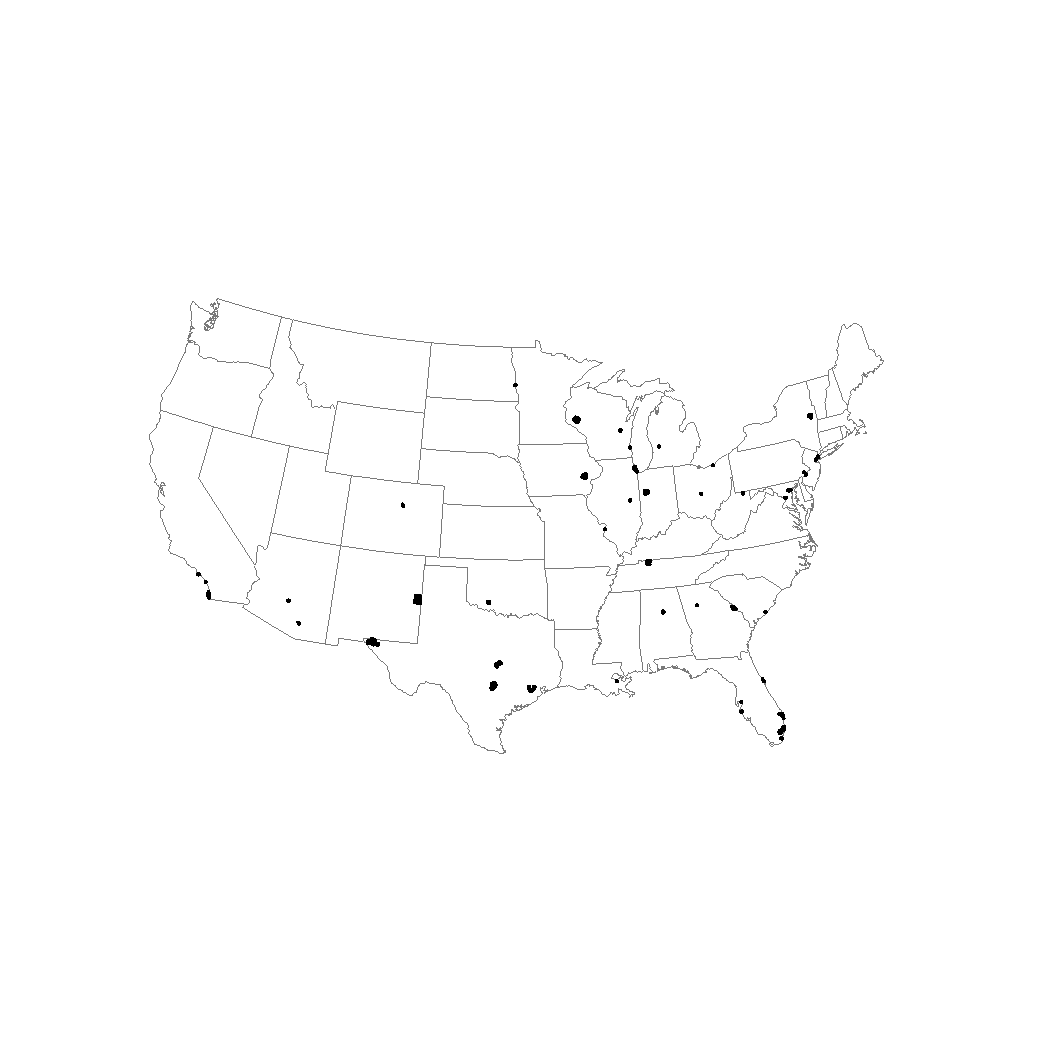
\includegraphics[scale=0.75]{figures/fig1a.pdf}   
 \flushleft
 Note: This figure shows ...
\end{figure}

%%%%%%%%%%%%%%%%%%%%%%%%%%%%%%%%
%   APPENDIX	 Tables	        %
%%%%%%%%%%%%%%%%%%%%%%%%%%%%%%%%
\pagebreak
\appendix
\renewcommand{\theequation}{\Alph{chapter}.\arabic{equation}}

\setcounter{figure}{0}
\setcounter{table}{0}
\makeatletter 
\renewcommand{\thefigure}{A.\@arabic\c@figure}
\renewcommand{\thetable}{A.\@arabic\c@table}

\section{Appendix: Tables and Figures}\label{sec:appendix_tables} 

\end{document}
